\documentclass[a4paper,10pt]{article}
\usepackage[utf8]{inputenc}
%\usepackage{fullpage}
\usepackage{graphicx}
\usepackage{rotating}

\usepackage{listings}
\lstset{
        basicstyle=\footnotesize,       % the size of the fonts that are used for the code
        numbers=left,                   % where to put the line-numbers
        numberstyle=\footnotesize,      % the size of the fonts that are used for the line-numbers
        stepnumber=10,                  % the step between two line-numbers. If it's 1, each line 
        breaklines=true,                % Wrap lines that are too long.
                                                                                                                                        % will be numbered
        numbersep=5pt,                  % how far the line-numbers are from the code
}

% Title Page
\title{CAP 6616 - Neuroevolution and Generative and Developmental Systems\\Midterm Report}
\author{Anthony Wertz \\ James Schneider}

\begin{document}
\maketitle

\section{Objective}

To evolve a neural network that provides unique transformations of human faces.

\section{Procedure}
\label{sec:procedure}

Using OpenCV we will detect a face in any image and transform the image for input to the neural network. First the input image will be passed to OpenCV, this open image processing library will be used to both detect and extract the face from the image in order to perform the transformation. After the image is extracted an interactive evolutionary process begins. The Neural Network scans through the image linearly with every x,y position of the output image being correlated to the position of a pixel from the original image in x,y. The network will then output the images to the user in a GUI format similar to how picbreeder functions. The user will choose an image from this GUI to further evolve and have the ability to save both the image and transformation function (evolved neural network).

This will be done using the HyperNEAT C++ software as a basis for executing the neuroevoltion process while using Python as the main means of processing the results and presenting the options to the user. The two languages will interact by providing Python bindings to the HyperNEAT code base. The interaction of the systems is depicted in figure \ref{fig:arch}.

% \begin{figure}
%     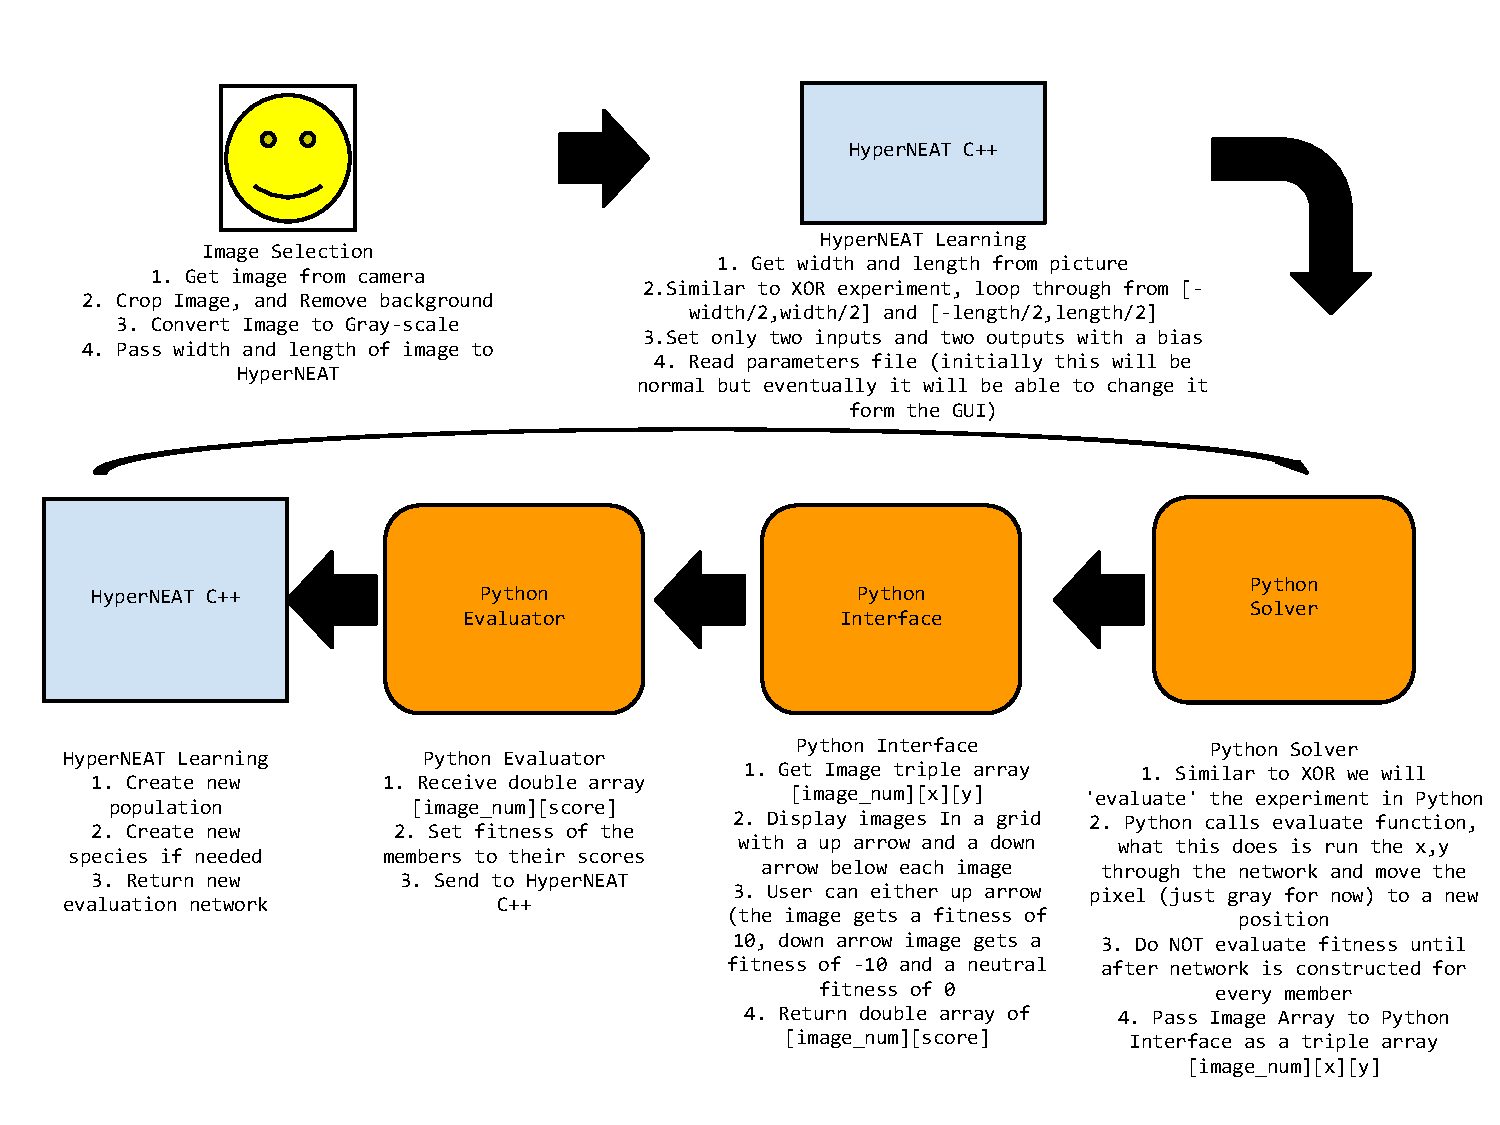
\includegraphics[width=\textwidth]{rec/arch.pdf}
%     \caption{Architecture}
%     \label{fig:arch}
% \end{figure}

As may be seen in figure \ref{fig:arch}, HyperNEAT C++ will be used to manage the interal processing of the main HyperNEAT components as that architecture already exists. However the Python system built will be used to display the population (through a GUI built with Qt), evaluate the viability of offspring (e.g. determine the fitness of population individuals via operator input), and send the results back to the HyperNEAT C++ layer for evolution.

An example of the GUI interface may be seen in figure \ref{fig:gui}. This figure shows the general layout where a user will be able to select an input image of a face and from there view and evolve the resulting outputs. A network distortion rasterizer has been built to utilize any given network representing a distortion in normalized coordinates to determine a new image. In the figure some dummy networks are shown which provide either a one to one pixel mapping or one or two dimensional flipping as a proof of concept, but in general each of the twelve figures would represent a different network that could be selected by the user for evolution.

In addition to the display as shown, evolution parameters will be avialable to the operator to change on the fly during evolution. The useful parameters have not yet been determined which is why they do not yet appear in the interface, but they will be added incrementally as the need arises during testing.

Current progress to this effect includes a large overhaul of the Python bindings available in the original HyperNEAT C++ code distribution to allow for Python tests to be built, the development of a new experiment module within HyperNEAT to support the necessary functionality, and the development of a graphical user interface to allow operator interaction with the evolutionary process. Most of the original work is presented in the source section in \ref{sec:source}, though some minor changes were omitted for brevity in this document.

\section{Questions}

Will image registration be required in order to generalize the evolved structure to many different images from any angle? How do you define the center of the picture, is it the nose feature’s centerpoint or the centerpoint of the bounding box? Do the features of the face improve the performance or detract? Should the evolved networks be seeded with symmetry or can this be found efficiently? Can the facial features be discovered and the neural network eventually understand the shapes of evolved nose structures and eye structures? Will the neural network allow for real time performance after evolution or should a transformation matrix be calculated in order to utilize the evolved image transformations?

\section{Output}

Standalone GUI with image evolution capabilities, image saving capabilities and neural network saving capabilities. This GUI will evolve a user’s image and allow the user to view each individual generation.

As described in section \ref{sec:procedure}, the GUI in figure \ref{fig:gui} is a representation of the operator interface.

\begin{figure}
    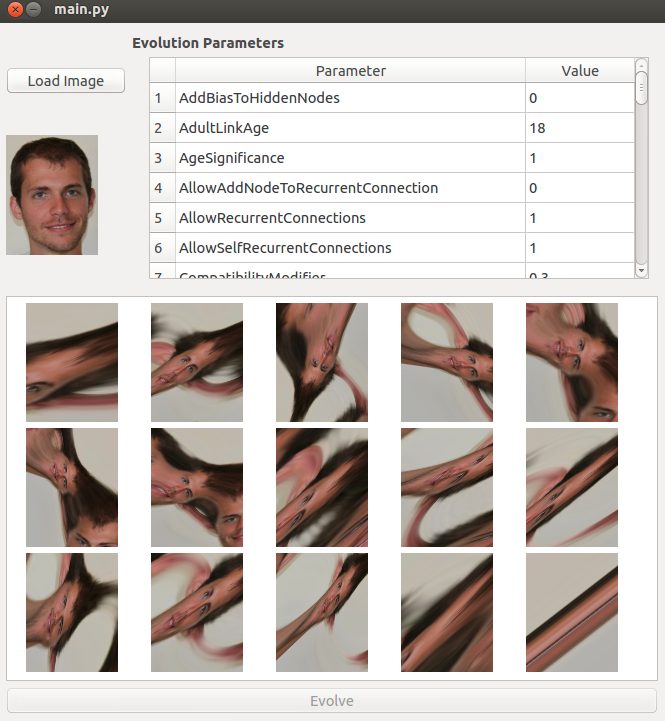
\includegraphics[width=\textwidth]{rec/gui.png}
    \caption{GUI Prototype}
    \label{fig:gui}
\end{figure}

\section{Software}

HyperNeat v4.0 C++ by Jason Gauci, pyQt framework v4.2.8 for GUI representation, OpenCV v 2.4, TinyXMLDLL v 2.0, JG template library, Boost C++, WxWidgets, GCC, Cygwin (windows Dev), Ubuntu (Linux Dev), CMake,Make, Python v 2.6

\section{Timeline and Work Distribution}

\begin{enumerate}
    \item 9/12 - 9/24: Get build environment working between Windows and Ubuntu (hyperNEAT and C++ bindings); use environment to build XOR using python.
Work Distribution: Independently get build working on respective platforms; independently implement XOR.
    \item 9/24 - 9/28: Build initial project architecture modules: (1) the python/hyperNEAT module that evolves CPPNs and sends the result to the user for evolution; (2) python/GUI module that displays the results sent by module 1, allows user selection, and returns the selection back to module 1 for further evolution.
Work Distribution: Collaboratively determine python interface between modules; independently build first pass of respective modules; collaboratively work on implementation.
    \item 9/28 - 10/3: Independently compile necessary documentation and graphics for respective modules; collaboratively compile documentation linking the two and considering the overall system architecture.
    \item 10/3 - 10/24: Experiment with evolution to attempt to evolve an interesting deformation (independently); through experimentation work out any software bugs; this is the baseline project implementation.
    \item 10/24 - 10/29: Consolidate interesting findings, issues, and experiences into the midterm report and presentation.
    \item 10/29 - 11/26: Use time as buffer to finish work on the baseline if good results weren’t obtained. If acceptable results were found, attempt to increase applicability and complexity by looking at extensions including: detecting image features to be used in the transform instead of just pixel locations; integrating evolved neural nets in a video (real time).
    \item 10/26 - 12/3: Consolidate final interesting results in a report and presentation.
\end{enumerate}

\section{Source Code}
\label{sec:source}

\subsection{PyHyperNEAT.cpp}
\lstinputlisting[language=C++]{../../external/HyperNEAT/NE/HyperNEAT/PyHyperNEAT/src/PyHyperNEAT.cpp}

%\subsection{HCUBE\_ExperimentRun.cpp}
%\lstinputlisting[language=C++]{../external/HyperNEAT/NE/HyperNEAT/HyperCube_NEAT/src/HCUBE_ExperimentRun.cpp}

\subsection{ImageExperiment.h}
\lstinputlisting[language=C++]{../../src/hyperneat/ImageExperiment/ImageExperiment.h}

\subsection{ImageExperiment.cpp}
\lstinputlisting[language=C++]{../../src/hyperneat/ImageExperiment/ImageExperiment.cpp}

\subsection{GUIWindow.py}
\lstinputlisting[language=Python]{../../src/gui/GUIWindow.py}

\subsection{PopulationModel.py}
\lstinputlisting[language=Python]{../../src/gui/PopulationModel.py}

\end{document}          
